\documentclass[11pt,a4paper]{article}

\usepackage[utf8]{inputenc}
\usepackage[T1]{fontenc}
\usepackage{amsmath}
\usepackage{amssymb}
\usepackage{booktabs}
\usepackage{graphicx}
\usepackage{hyperref}
\usepackage{url}
\usepackage[margin=1in]{geometry}

\hypersetup{
  colorlinks=true,
  linkcolor=black,
  citecolor=black,
  urlcolor=blue
}

\title{Aggregate Ranking Metrics Can Invert Operational Order:\\
An Alert-Budget-Constrained Benchmark for\\
Authentication Anomaly Detection}

\author{Mahamane Sani Adamou Mahamane\\
\small \texttt{saniadamou778@gmail.com}\\
\small AuthBench: \url{https://github.com/SaniAdamou14/AuthBench}}

\date{September 2026}

\begin{document}
\maketitle

\begin{abstract}
A security operations centre can triage a few dozen alerts per analyst per day.
Most published anomaly-detection results are reported at operating points no
analyst could ever staff. We present \textbf{AuthBench}, a leak-free,
alert-budget-constrained benchmark for authentication-log anomaly detection, and
report its first results on real data from the Los Alamos National Laboratory
(LANL) Comprehensive Multi-Source Cyber-Security Events dataset.

On a test day of 19{,}870{,}848 authentication events containing 39 real
red-team campaigns, \emph{no} model detects a single campaign at 10, 50 or 100
alerts per day: six of the seven measurably so, the seventh being a
degenerate floor whose result is undetermined for a reason we report. One model
catches two campaigns at 500 alerts per day, a budget no SOC staffs. More
consequentially, the two evaluation registers are not merely different but
\textbf{anti-correlated}: the model with
the best ROC-AUC (0.942) detects nothing at any budget, while the only model that
detects anything has the lowest ROC-AUC of the five non-trivial models (0.547).
Ranking these models by the literature-comparable metric would place the model
that detects nothing first and the only model that detects something last.

We also report a control that we believe generalises beyond this benchmark. On a
synthetic sample, the same rule-based model reaches 100\% campaign recall at a
budget of 10, but a measured rule-level decomposition shows that a single rule
implementing the same predicate as the data generator carries $113\times$
separation and 0.521 of the model's fitted weight. Against a red team that never
read the rules, that model falls to 5.1\%. A synthetic benchmark cannot establish
whether a heuristic is good or merely well-informed.

We state the binding limitations explicitly, including one that biases in the
direction that flatters our own conclusion. The benchmark proposes no new model;
it measures what survives a realistic operating point.
\end{abstract}

\section{Introduction}

Anomaly detection in authentication logs has an uncomfortable disconnect at its
centre: the metric a paper reports and the protection an organisation actually
receives can point in opposite directions.

The mechanism is not subtle. Authentication telemetry in an enterprise network
carries positive rates on the order of $10^{-5}$ to $10^{-7}$. At that base rate,
a classifier that always predicts ``benign'' achieves accuracy above 99.9999\%,
and a ranking metric computed over the full period can remain high for a model
whose highest-ranked events on any given day contain no attack at all. Axelsson's
base-rate argument~\cite{axelsson2000} made this point for intrusion detection a
quarter-century ago; Sommer and Paxson~\cite{sommer2010} made it for machine
learning specifically. The field has continued to report aggregate metrics
anyway.

What is missing is not the argument but the measurement. This paper contributes
a benchmark built so that the measurement is possible:

\begin{enumerate}
  \item \textbf{A dual-register evaluation.} Every model is scored both in a
  \emph{literature-comparable} register (ROC-AUC, global precision@$k$, recall at
  fixed FPR; reported so results can be placed next to published ones, never
  to rank models) and in an \emph{operational} register (AUC-PR, per-campaign
  recall at a fixed \emph{daily} alert budget, time-to-detection, and budget for
  first detection).

  \item \textbf{A strictly temporal, leak-free protocol} with mechanical
  enforcement: a split guard that raises on any ordering violation, an
  architecture test forbidding model and feature code from importing the
  test-partition loader, and causal windowing primitives that exclude the current
  event's own timestamp.

  \item \textbf{The measured result on real attacks}, reported in
  Section~\ref{sec:results}: at any operational budget, the two registers are
  anti-correlated.

  \item \textbf{A circularity control} (Section~\ref{sec:circularity}) showing
  that the same benchmark run on a synthetic sample produces a result that is
  largely an artifact of the generator sharing a predicate with the model.
\end{enumerate}

We deliberately do not propose a new detector. The benchmark's claim is about
evaluation, and a new model would only invite the reader to evaluate \emph{it} by
the metrics we are arguing against.

\section{Background and related work}

\paragraph{The critique is classical.}
Axelsson~\cite{axelsson2000} established the base-rate fallacy for intrusion
detection: at realistic base rates, even very low false-positive rates yield
alert streams dominated by false alarms. Sommer and Paxson~\cite{sommer2010}
extended the argument to machine-learning-based detection and received the IEEE
S\&P Test of Time Award in 2020 for it. More recently, TESSERACT~\cite{tesseract}
and Arp et al.~\cite{arp2022} named temporal snooping and base-rate neglect as
recurring, specific methodological errors in security machine learning, with
measured consequences for reported performance.

Our contribution is not to restate these arguments but to build an evaluation
harness in which their consequences are measured on real red-team activity, and
to report what happens to a model catalogue under that harness.

\paragraph{Detection on the LANL dataset.}
The LANL Comprehensive Multi-Source Cyber-Security Events
dataset~\cite{kent2015} is among the few public corpora pairing real enterprise
authentication telemetry with labelled red-team activity. Two methodologically
distinct lines of work use it. Tuor et al.~\cite{tuor2018} apply recurrent
neural network language models at the event level, reporting up to 0.876 ROC-AUC
and 87.0 average precision at user-day granularity, and up to 0.98 ROC-AUC at
event granularity for their character-level model. Turcotte et
al.~\cite{turcotte2016} take a peer-based approach, using Poisson factorisation
to identify anomalies relative to comparable user groups rather than relative to
an individual's own history.

In Tuor et al.'s reported results, ROC-AUC and average precision move together
across all ten configurations; no divergence comparable to the one we report
appears. We do not read this as a contradiction. Their operational metric,
average daily percentile, is continuous and forgiving, not a recall
constrained to a fixed daily alert budget corresponding to an analyst's real
quota. The divergence we measure is a property of the operating point, and it is
visible only when the operating point is imposed.

To our knowledge, no published work on LANL reports a budget-constrained
operational metric alongside the standard aggregate metric on the same models.

\section{Dataset, labelling and campaign construction}

\subsection{Source}

We use the LANL authentication log (\texttt{auth.txt.gz}, SHA-256
\texttt{9c6b0cc2\ldots f672}, 7{,}626{,}505{,}158 bytes), containing
1{,}051{,}430{,}459 authentication events over 58 days from one enterprise
Windows/Active Directory environment in 2015.

Several dataset quirks are handled explicitly rather than silently. The
\texttt{auth\_type} field is null for approximately 55\% of events and
\texttt{logon\_type} for approximately 14\%; the \texttt{?} sentinel is converted
to a dedicated boolean rather than imputed. Timestamps begin at epoch 1 with
one-second resolution and no timezone, so the night window used by temporal
features is calibrated empirically from the training split rather than assumed.
Machine accounts (\texttt{\$} suffix) constitute most of the volume and are
flagged, never dropped or coerced. Failure events exist only for users who
succeeded somewhere, so no conclusion is drawn about brute-force activity against
nonexistent accounts.

\subsection{Labelling}

Red-team labels are joined on the full quadruplet
$(\textit{time}, \textit{user}, \textit{domain}, \textit{src\_computer},
\textit{dst\_computer})$, never on time alone: a looser join silently inflates
the positive count. The pipeline additionally asserts that the observed positive
rate falls inside a configured range and aborts otherwise.

\subsection{From events to campaigns}

The red-team file contains 749 raw rows. After removing 34 exact duplicates
(\textbf{measured on the file}, rather than adopting the widely repeated secondary
figure of 737), 715 distinct red-team events remain.

These are not 715 independent attacks. They are a small number of
lateral-movement campaigns, and evaluating per-event recall would both overstate
the number of independent successes and understate the operational question,
which is whether the \emph{intrusion} was caught at all. We therefore group
events into campaigns by \texttt{user@domain} with a configurable gap threshold
(\texttt{campaign\_gap\_hours}, default 24 hours).

No canonical grouping exists in the literature. The sensitivity of the resulting
campaign count to this threshold is therefore a required analysis, not a
decorative one, and is treated as such by the specification.

\section{Protocol}

\subsection{Temporal split, and why it is one day per partition}
\label{sec:split}

\begin{table}[t]
\centering
\begin{tabular}{lrrrr}
\toprule
Partition & Day & Events & Positives & Campaigns \\
\midrule
Train      & 5  & 18{,}557{,}382 & 21  & 4  \\
Validation & 8  & 19{,}374{,}688 & 261 & 45 \\
Test       & 12 & 19{,}870{,}848 & 207 & 39 \\
\bottomrule
\end{tabular}
\caption{The evaluated split. One day per partition, non-contiguous, over
converted days 0--13 (239{,}471{,}459 events). Test positive rate:
$1.04 \times 10^{-5}$.}
\label{tab:split}
\end{table}

The split is shown in Table~\ref{tab:split}. It is one day per partition and
skips the days between. This requires explanation, because it is not the split
the specification originally proposed.

The natural contiguous split (train days 0--29, validation 30--39, test 40--57)
\textbf{cannot be run at all}. The red team stops at day 29. That split
places every red-team event in the training partition and leaves validation and
test with no positives whatsoever: every ranking metric would be undefined, and
the rule model's weight calibration would have nothing to maximise. A unit test
refuses any split that repeats this error.

Three constraints do admit a solution simultaneously: campaigns must be present
in every partition; temporal order must hold ($5 < 8 < 12$); and no partition may
exceed roughly 20M events without exhausting the 8\,GB reference machine.
Days 0, 3, 4, 10 and 11 contain no red-team activity inside the converted window,
which further constrains the choice.

The gaps between partitions are not leakage (nothing from day 6 or day 9
reaches any model), and testing on day 12 after training on day 5 is a
\emph{harder} generalisation test than testing on the following day would be.
What the choice costs is one day of history per partition, which is the binding
limitation on every number in this report and is discussed in
Section~\ref{sec:threats}.

\subsection{Leakage control}

Three mechanisms enforce the temporal protocol rather than documenting it:

\begin{itemize}
  \item \texttt{verify\_temporal\_order} raises \texttt{LeakageError} unless
  $\max(\textit{train.time}) < \min(\textit{val.time})$ and
  $\max(\textit{val.time}) < \min(\textit{test.time})$.

  \item An architecture test forbids any module under \texttt{models/} or
  \texttt{features/} from importing the test-partition loader.

  \item All windowed features are computed through causal primitives: rolling
  aggregations use a left-closed window $[t - w, t)$ that excludes the current
  event's own timestamp, and statistics a running sum cannot express (distinct
  counts, entropy) use a self-join restricted to strictly prior events of the
  same entity. A unit test constructs synthetic events whose feature value would
  differ if the future were visible, and asserts the computed value is the causal
  one.
\end{itemize}

\subsection{Fitted quantities}

Two quantities in the feature pipeline are learned rather than computed
row-locally: the night window, and the frequency encoding of categorical event
fields. Both are fitted on the training split only and applied unchanged to
validation and test.

Fitting either per-split is a leak that produces no error and no warning: it
allows an event's encoding to depend on events that came after it, and assigns
the same \texttt{auth\_type} different numeric values in train and test. The
feature function therefore takes the fitted encoding as a \emph{required}
argument. A protocol that depends on the caller remembering an optional keyword
is not a protocol.

\section{Model catalogue}
\label{sec:models}

Seven models were evaluated, from a catalogue of eight:

\begin{itemize}
  \item \textbf{M0a random} and \textbf{M0b always-fail}: floors, present so
  that every reported number has a reference point that cannot be beaten by
  accident.
  \item \textbf{M1 rules}: seven hand-written detection rules with weights
  calibrated on the validation split.
  \item \textbf{M2a pair rarity}: a statistical novelty score over
  (source, destination) authentication pairs.
  \item \textbf{M2b PCA reconstruction}: reconstruction error under a
  principal-component model.
  \item \textbf{M3a Isolation Forest} and \textbf{M3b HBOS}: standard
  unsupervised outlier detectors.
\end{itemize}

The eighth, \textbf{M3b ECOD}, was excluded: its scoring raised
\texttt{MemoryError} at 3.89\,GiB, because the implementation concatenates the
fitted sample onto the frame being scored and argsorts all columns of the result.
This is a property of the model, not of the harness, and it has a second
consequence worth stating: ECOD is transductive, so an event's score depends on
which other events are scored alongside it: the same row scores 10.64 alone
and 10.81 among four hundred others. No label crosses the train/test boundary, so
this is not leakage in the sense our guards address, and it is how ECOD is used
in the literature. But a benchmark claiming a strictly temporal protocol owes its
reader that sentence rather than leaving it in a library's source. This was found
by a test asserting the opposite property: that scoring a split piecewise
gives the same answer as scoring it whole.

\paragraph{No deep-learning model is evaluated here.} Feature families for graph
and sequence structure, and the corresponding deep and graph models, are
implemented and unit-tested but are not part of the default pipeline and were not
run on LANL. The question of how much deep learning buys over well-built
heuristics at a realistic operating point is the question this benchmark is
built to ask; it is not a result this report claims to answer.

\section{Evaluation: two registers}

Metrics are kept in two registers under separate keys, and the report generator
cannot mix them.

\paragraph{Operational.} AUC-PR with campaign-stratified confidence intervals is
the headline ranking metric. Recall at alert budget takes the top-$k$ scored
events \emph{per day}, never top-$k$ over the whole period, and is reported both
per event and per campaign. Time-to-detection counts campaigns never detected at
a given budget in the denominator; they are never dropped and never folded in as
a delay of zero.

\paragraph{Budget for first detection.} A recall table reading $0\%\ 0\%\ 0\%\
0\%$ ranks every failed model as equally far from working. A model whose best
campaign sits at rank 600 and one whose best sits at rank 9{,}000{,}000 print
identically, and that is precisely the regime this benchmark studies. We
therefore also report the smallest daily budget at which a model detects any
campaign, computed exactly as the minimum rank over campaign events within their
own day. On the synthetic sample it separates four models that the recall row
called identical (83 / 114 / 284 / 294) and reveals that two of them lose to the
random floor.

We note the obvious objection: this metric was designed for exactly the regime
the LANL run occupies, and yet no LANL values are reported for it. The reason is
provenance, not selection. \textbf{The metric postdates the committed LANL run},
as do the tie-break fix of Section~\ref{sec:threats} and the score-resolution
diagnostics; that snapshot is frozen, and re-running it is precisely what the
history limitation makes expensive. Reporting the metric on the synthetic sample
only, and saying so, seemed better than either omitting it (it is part of the
protocol being described) or quietly recomputing it against a run whose
published tables would then no longer match the code.

\paragraph{Tie-breaking, stated rather than inherited.} ``The top 10 events of
the day'' is not a question a coarse-scored model answers on its own: the
always-fail floor puts 2{,}619 equally-scored events in competition for 8 places
on the demo sample. Equal scores are ordered by $(\textit{time},
\textit{event\_id})$: arrival order, label-free and total. Before this was made
explicit, ties fell to the frame's row order, which is alphabetical by user; the
consequence for our own published floor row is reported in
Section~\ref{sec:threats}. A zero-width tie bracket now certifies that the
tie-break decided nothing, which is the case for every model whose score is
continuous.

\paragraph{Literature-comparable.} ROC-AUC, global precision@$k$ (top-$k$ over
the whole period, as the literature reports it, which is \emph{not} the per-day
operating point), and recall at fixed FPR. ROC-AUC always emits an explicit
warning in the output, because it stays high for operationally useless models at
this base rate. These numbers exist so results can be placed beside published
ones. They are never used to rank.

\section{Uncertainty quantification}
\label{sec:uncertainty}

A single campaign-stratified resampling pass evaluates every model on each
resample, yielding both per-model confidence intervals and every pairwise
difference from the same sampling distribution. Each difference is therefore
paired: campaign-composition noise cancels between two models rather than being
counted twice.

Three artifacts of this method can manufacture a verdict indistinguishable from a
real one. All three are handled explicitly, and we report them because each one
would have flattered our results if left alone:

\begin{itemize}
  \item \textbf{Degenerate resamples.} A ranking metric over zero positives is
  undefined, but the underlying library returns $0.0$, so every model ties, and
  ties count in both tails. With one campaign in a split, roughly 37\% of
  resamples are degenerate, flooring $p$ near 0.74. Degenerate resamples are
  discarded and redrawn, and the count is reported.

  \item \textbf{Bootstrap resolution versus Holm.} A percentile bootstrap cannot
  report $p$ below $2/(R+1)$, while Holm's strictest threshold is
  $\alpha / n_{\text{pairs}}$. For an eight-model catalogue this requires
  $R \geq 1119$; the original configuration of 1000 resamples could never have
  yielded a significant result. The bound is computed rather than assumed, and
  the configuration now uses $R = 2000$.

  \item \textbf{A single campaign.} The sample size of a campaign-stratified
  bootstrap is the number of \emph{campaigns}. With one, every resample
  re-weights the same attack, no pairwise difference changes sign, and every
  $p$-value lands on $2/(R+1)$, below Holm's threshold, so every comparison
  reads ``outperforms''. The synthetic sample produced 21 out of 21 verdicts this
  way. A minimum of two campaigns is now required before any significance verdict
  is reported; point estimates and intervals are unchanged, only the verdict is
  withheld.
\end{itemize}

\section{Results}
\label{sec:results}

\begin{table}[t]
\centering
\small
\begin{tabular}{lrrrrrr}
\toprule
Model & AUC-PR [95\% CI] & ROC-AUC & @10 & @50 & @100 & @500 \\
\midrule
M0a random \emph{(floor)}        & 0.00001 [0.00000, 0.00002] & 0.500 & 0\% & 0\% & 0\% & 0\% \\
M0b always-fail \emph{(floor)}$^\dagger$ & 0.00001 [0.00000, 0.00002] & 0.496 & --- & --- & --- & --- \\
\textbf{M2a pair rarity}         & \textbf{0.00065} [0.00023, 0.00131] & \textbf{0.942} & 0\% & 0\% & 0\% & 0\% \\
M2b PCA reconstruction           & 0.00005 [0.00002, 0.00011] & 0.893 & 0\% & 0\% & 0\% & 0\% \\
M3a Isolation Forest             & 0.00004 [0.00001, 0.00010] & 0.872 & 0\% & 0\% & 0\% & 0\% \\
M3b HBOS                         & 0.00005 [0.00002, 0.00012] & 0.875 & 0\% & 0\% & 0\% & 0\% \\
M1 rules                         & 0.00010 [0.00002, 0.00071] & 0.547 & 0\% & 0\% & 0\% & \textbf{5.1\%} \\
\bottomrule
\end{tabular}
\caption{Results on the LANL test day. Campaign recall at daily alert budgets of
10, 50, 100 and 500. $^\dagger$M0b's budget columns are \emph{undetermined}
rather than zero; see Section~\ref{sec:threats}.}
\label{tab:results}
\end{table}

Table~\ref{tab:results} reports the run, and Figure~\ref{fig:recall} plots it.
Two findings follow.

\begin{figure}[t]
\centering
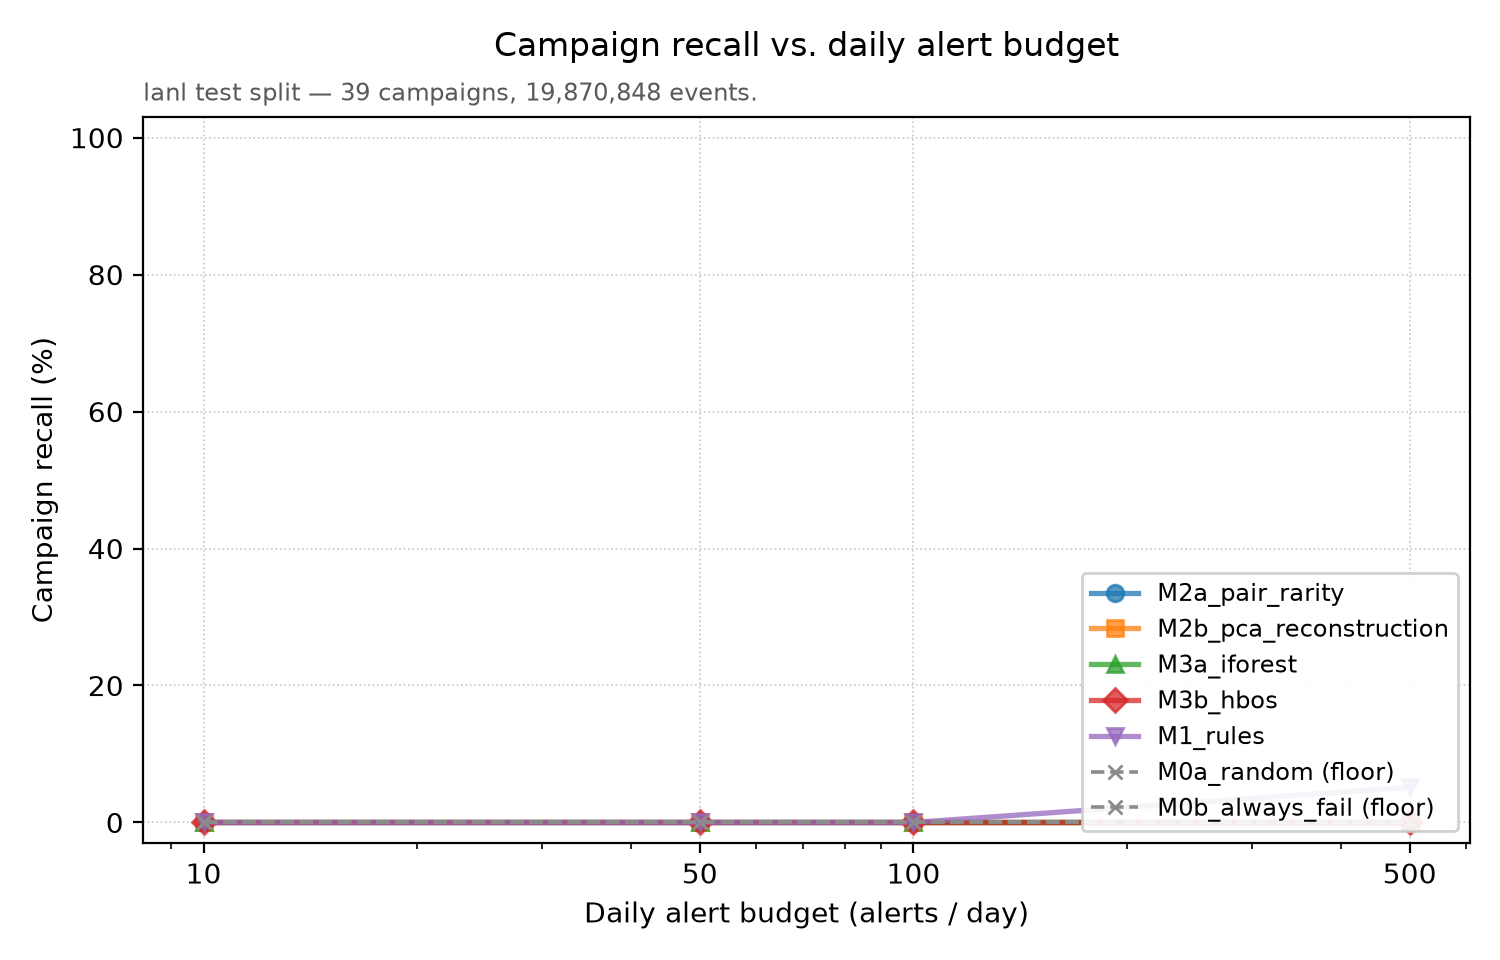
\includegraphics[width=0.92\textwidth]{campaign_recall_vs_budget.png}
\caption{Campaign recall against daily alert budget on the LANL test day,
reproduced as generated. Every curve lies on zero across the entire budget
range; the single departure is the rule model reaching 5.1\% at 500 alerts per
day, in the lower right. The emptiness of the plot is the result, not a
rendering failure. (The generated legend overlaps that one departure; this is a
cosmetic defect of the plotting code, left uncorrected here so that the figure
matches the committed output byte for byte.)}
\label{fig:recall}
\end{figure}

\subsection{Nothing works at an operational budget}

No model detects a single campaign out of 39 at 10, 50 or 100 alerts per day.
Six of the seven are measured at exactly zero; the seventh, the always-fail
floor, is undetermined at every budget for a reason given in
Section~\ref{sec:threats}; and, being a degenerate floor, any nonzero recall it
showed would be an artifact of alert ordering rather than detection. One model
(the rule-based heuristic) catches two campaigns at 500 alerts per day, a
budget no SOC staffs for a single analyst.

\subsection{The registers are anti-correlated, not merely different}

This is the benchmark's reason to exist, and it appears here on real attacks:

\begin{itemize}
  \item \textbf{M2a scores ROC-AUC 0.942 and detects nothing} at any operational
  budget. A ROC-AUC of 0.94 passes without comment in a paper.
  \item \textbf{M1 has the lowest ROC-AUC of the five non-trivial models,
  0.547} (barely above the 0.50 the floors score by construction) and is the
  only model that catches anything at all.
\end{itemize}

Ranking the non-trivial models by the literature-comparable metric would place
the model that detects nothing first, and the only model that detects something
last. This is not a claim that the weak model is better: it is a claim that the
ordering induced by the aggregate metric carries no information about the
ordering that matters operationally, and on this data inverts it.

\subsection{What the significance testing does and does not establish}

Thirteen of the 21 pairwise comparisons are significant after Holm-Bonferroni
correction. \textbf{Twelve of those thirteen are bounds, not measurements.} No
resample out of 2000 placed the difference on the other side of zero, so their
$p$-value is the bootstrap's own resolution floor and they are reported as
Holm-adjusted $p \leq 0.0210$ against a threshold of 0.05; true, with a factor
of 2.4 in hand, but not a value the run resolved. The single exception, and the
only pairwise verdict here whose $p$-value the bootstrap actually measured, is
M0b always-fail versus M1 rules at Holm-adjusted $p = 0.0450$.

Two non-results are worth as much as the significant ones. \textbf{M2a versus M1
is not significant} (Holm-adjusted $p = 0.828$; raw $p = 0.138$), and neither is
M1 versus the random floor (Holm-adjusted $p = 0.176$; raw $p = 0.022$). We are
therefore \emph{not} claiming that the rule model outperforms the statistical
one. The claim is about the divergence between registers, which does not require
either model to beat the other.

\section{A control for circularity}
\label{sec:circularity}

The same protocol was run on a synthetic sample before the real data, and the
comparison between the two runs is, in our view, a result in its own right.

On the synthetic sample, M1 reached \textbf{100\% campaign recall at a budget of
10}. Taken alone, this would support a clean narrative: well-built heuristics beat
every machine-learning model at every budget.

The narrative does not survive a rule-level decomposition
(Table~\ref{tab:rules}). The generator emits each campaign as a chain (the
user authenticates $A \to B$, then $B \to C$), and rule R7 tests for exactly
that: previous destination equals current source, within 30 minutes. The
generator and the rule implement \textbf{the same predicate}. R7 separates
malicious from benign by a factor of $113\times$, and the validation-fitted
weights place 0.521 on it, more than half the model's score.

\begin{table}[t]
\centering
\begin{tabular}{lrrr}
\toprule
Rule & Mean score, benign & Mean score, malicious & Ratio \\
\midrule
\textbf{R7 lateral chain} & 0.0056 & 0.6364 & $\mathbf{113\times}$ \\
R6 new auth type          & 0.1539 & 0.5455 & $3.5\times$ \\
R1 new pair               & 0.3950 & 1.0000 & $2.5\times$ \\
R4 off-hours              & 0.7237 & 0.6406 & $0.9\times$ \emph{(none)} \\
R2 / R3 / R5              & ---    & 0.0000 & never fire \\
\bottomrule
\end{tabular}
\caption{Rule-level discrimination on the synthetic sample. Generated output,
regenerated by every run and covered by the reproducibility check, so the caveat
cannot quietly stop matching the run it describes.}
\label{tab:rules}
\end{table}

This is a property of a synthetic sample written by the same author as the rules,
not a finding about heuristics, and no amount of statistical care fixes it. A
campaign-stratified bootstrap will faithfully report a circular result with
correct confidence intervals.

\textbf{The LANL run is the control, and it confirms the diagnosis.} Against a
red team that never read R7, the same model falls from 100\% at budget 10 to
5.1\% at budget 500 and 0\% everywhere else.

We state the general form deliberately, because we think it is the most
transferable thing in this report: \emph{a synthetic benchmark cannot tell you
whether your heuristic is good or merely well-informed; only an adversary who did
not read your rules can.}

\section{Threats to validity}
\label{sec:threats}

\subsection{One day of history per partition}

Each partition is a single day with no warm-up, so 24-hour window features and
cumulative pair statistics see at most one day of past inside their own
partition.

This makes a campaign recall of 0\% ambiguous between two readings that this run
cannot separate: either the models genuinely detect nothing at an operational
budget, or one day is insufficient history to establish what counts as
\emph{new}, and the novelty features carrying the lateral-movement signal are
being measured against a past that barely exists.

The size of the effect is measured rather than guessed. On the synthetic sample,
adding two warm-up days halves the count of pairs flagged as never-seen
($2{,}623 \to 1{,}287$) over an identical set of written events, raises mean pair
rarity from 7.00 to 7.73, and raises mean per-user daily event count from 7.85 to
10.33. Without history, half the pairs called ``never seen before'' were only
unseen because there was no past in which to have seen them.

The warm-up parameter exists and works; the reference machine cannot afford it.
One warm-up day makes each split process 38M rows instead of 19M and the run died
after writing the first split; two makes it 57M and it died before writing
anything.

\textbf{What this limitation does not reach} is the anti-correlation itself. That
M2a at 0.942 detects nothing while M1 at 0.547 detects something is a property of
the operating point and the base rate, and no quantity of history changes it.

\subsection{A robustness check: the wider window, with warm-up}
\label{sec:wider-window}

The limitation above is no longer entirely hypothetical. A second run, on
hardware large enough to afford what the reference machine could not, trains
on days 0--7, validates on 8--10 and tests on 11--13, with two warm-up days
feeding every split's first events a real past (133{,}093{,}586 /
51{,}687{,}105 / 54{,}690{,}768 rows; 52 test-split campaigns against the
single day's 39). Full output: \texttt{reports/lanl/wider\_window\_results/}.

The central finding is unchanged, and if anything sharper. Every one of the
seven scoreable models (M3b ECOD excluded here for the same reason given
in Section~\ref{sec:models}, at larger scale) reads exactly 0\% campaign
recall at every budget from 10 through 500 alerts per day, over 52 campaigns
rather than 39. The anti-correlation holds too: M2a's ROC-AUC is 0.941
(0.942 on the single day) against zero operational recall, to three figures
the same finding from a test split more than five times the size.

One number does move, and it is reported here rather than only the numbers
that confirm the paper's thesis. M1 rules (Table~\ref{tab:results}'s only
non-zero row, 5.1\% campaign recall at 500 alerts/day) reads 0\% on the
wider run, at every budget. Two things changed together between the runs,
not one: three test days instead of one, and warm-up switched on for the
first time on real data. Section~\ref{sec:threats}'s own measurement above is
that warm-up roughly halves how often a pair is flagged never-seen-before;
M1's R1 and R6 rules are built directly on that signal. A plausible reading
is that warm-up did here what it was already shown to do on the synthetic
sample: shrink the over-flagging that let M1 catch two campaigns on an
unwarmed-up test day, rather than three days being harder to detect in
than one. \textbf{This is not isolated}: separating window width from
warm-up would need a third run holding one fixed, which is future work, not
a claim made here.

\subsection{Cold start is encoded as ``normal'', and it biases toward our conclusion}

An event with no prior history for its user does not receive a neutral feature
value: it receives the most normal one available. The hour-deviation feature is
filled with $0.0$ for a user's first event in a partition, and $0.0$ is the
\textbf{minimum} of that column's range; the failure-ratio features are likewise
0 when there are no prior events to have failed.

Measured on the synthetic test split rather than asserted: 3{,}299 of 8{,}049
events (41\%) have no prior one-hour history; 350 events are a user's first in
the split, and all 350 (and no other event) carry the sentinel value,
against a median deviation of 0.426 elsewhere and a 99th percentile of 3.046. Two
of eleven malicious test events fall in that set.

The sentinel and the cold-start set coincide exactly, and those events are scored
as maximally typical on that axis. This is the same history shortage seen from the
feature side, and the shorter each partition, the larger the affected share.
\textbf{It biases in the direction that produces the reported zeros, which is the
direction that flatters our conclusion}, so we state it here rather than leave it
to be found.

It is not fixed, and the reason is a trade rather than an oversight: changing the
sentinel changes the design matrix, which moves every vector-space model's scores
and would desynchronise the published snapshot from the code that claims to
produce it. The honest options (a cold-start indicator column, or a sentinel
outside the column's range) are changes to the protocol and belong with a
re-run.

\subsection{One floor row is undetermined rather than zero}

M0b always-fail scores every event 0 or 1, so on a 19.9M-event test day its alert
set at any budget is decided entirely by how equally-scored events are ordered.
The published run used the ordering then in force: the frame's own row order,
alphabetical by user. \textbf{M0b's zeros are therefore a property of that
ordering, not of the floor}, and should be read as undetermined. On the synthetic
sample, the tie-break fix moved M0b from 0\% to 75\% at budget 500.

Every other row is unaffected: their scores are continuous and leave the
tie-break nothing to decide. Nothing here touches AUC-PR, ROC-AUC, the confidence
intervals or the pairwise comparisons, none of which depend on alert ordering.

\subsection{Remaining threats}

\begin{itemize}
  \item \textbf{A single real dataset.} LANL describes one enterprise network, in
  2015, on Windows/Active Directory. Nothing here establishes transferability to
  a modern cloud or hybrid environment.

  \item \textbf{Dataset age.} Eleven years old at the time of writing.
  Authentication patterns have shifted: widespread MFA, token-based
  authentication. The \emph{protocol} remains valid; absolute performance numbers
  are not transferable to present-day environments.

  \item \textbf{Incomplete labels.} Red-team events are a partial ground truth.
  An event not flagged as red-team may still be an undetected real compromise
  from 2015, so a ``false positive'' here may be an unlabelled true positive.
  Precision figures should be read with that caveat.

  \item \textbf{No adaptive adversary.} The LANL red team was not attempting to
  evade these specific models. Reported numbers are an optimistic upper bound
  against an adversary who knows they are being watched by exactly this stack.

  \item \textbf{Campaign-grouping sensitivity.} Campaign-level recall depends on
  the grouping gap threshold, for which no canonical value exists.
\end{itemize}

\section{What this benchmark does not show}

We are explicit about the boundary of the claim, because the result is easy to
overstate.

It does \textbf{not} show that anomaly detection on authentication logs is
hopeless. It shows that seven specific models, under one specific protocol, with
one day of history, on one day of one 2015 network, detect nothing at a budget an
analyst could staff.

It does \textbf{not} show that deep learning fails at this task: no
deep-learning model was evaluated here (Section~\ref{sec:models}).

It does \textbf{not} show that heuristics beat learned models: the comparison
between the rule model and the statistical one is explicitly not significant
(Section~\ref{sec:results}).

What it does show is narrower and, we argue, more useful: that on this data the
ordering induced by the standard aggregate metric is not merely uninformative
about operational value but inverted with respect to it, and that a benchmark
reporting only the aggregate metric would have ranked the single model that
detected anything last.

\section{Reproducibility}

The pipeline is staged (\texttt{ingest} $\to$ \texttt{parse/clean} $\to$
\texttt{label} $\to$ \texttt{split} $\to$ \texttt{features} $\to$
\texttt{models} $\to$ \texttt{evaluate} $\to$ \texttt{report}), each stage a pure
function over lazy frames, with data-version control over inputs and outputs and
experiment tracking over runs. Continuous integration runs linting, strict type
checking and the test suite on every change, with a coverage gate on the
evaluation and feature modules.

The protocol is written against the full 1.05-billion-event corpus. Five changes
brought a full run from roughly 161\,GB of disk and 439\,GB of RAM down to
roughly 81\,GB and 49\,GB (a day-window conversion, a feature store projected
to the columns actually read, bounded-sample fitting, day-chunked scoring, and a
rank-ordered bootstrap), and none of them moves a measured number: the
synthetic report regenerates byte for byte after all five. A preflight command
prints the budget for the machine it runs on and exits non-zero when the run does
not fit, naming the event count that would.

On the reference machine (8\,GB RAM, 6 cores): conversion 2.5 minutes, feature
build 18 minutes, evaluation 5 hours 20 minutes before the bootstrap was
parallelised; the bootstrap itself went from 4h49 on one core to roughly 1h15 on
four, with bit-identical results.

Code, configuration and the committed report outputs are available at
\url{https://github.com/SaniAdamou14/AuthBench}.

\section{Conclusion}

We built a benchmark to ask whether reported anomaly-detection performance
survives a realistic alert budget, and measured the answer on real red-team
activity. It does not: none of seven models detects any of 39 campaigns at 10, 50
or 100 alerts per day. The sharper finding is that the standard aggregate metric
does not merely fail to predict operational value on this data: it inverts the
ordering, placing a model that detects nothing above the only model that detects
anything.

We also showed, by running the same protocol on a synthetic sample, that a
heuristic can appear to dominate for reasons entirely internal to the data
generator, and that only an adversary who did not read the rules can distinguish
a good heuristic from a well-informed one.

The most useful next steps are, in our view, a run with adequate history per
partition (the binding limitation on every number reported here) and the
evaluation of sequence and graph models under the same budget constraint, so that
the question the benchmark was built to ask can finally be answered rather than
posed.

\begin{thebibliography}{9}

\bibitem{axelsson2000}
S.~Axelsson.
\newblock The base-rate fallacy and the difficulty of intrusion detection.
\newblock \emph{ACM Transactions on Information and System Security}, 3(3):186--205, 2000.

\bibitem{sommer2010}
R.~Sommer and V.~Paxson.
\newblock Outside the closed world: On using machine learning for network intrusion detection.
\newblock In \emph{IEEE Symposium on Security and Privacy}, 2010.

\bibitem{tesseract}
F.~Pendlebury, F.~Pierazzi, R.~Jordaney, J.~Kinder, and L.~Cavallaro.
\newblock TESSERACT: Eliminating experimental bias in malware classification across space and time.
\newblock In \emph{USENIX Security Symposium}, 2019.

\bibitem{arp2022}
D.~Arp, E.~Quiring, F.~Pendlebury, A.~Warnecke, F.~Pierazzi, C.~Wressnegger, L.~Cavallaro, and K.~Rieck.
\newblock Dos and don'ts of machine learning in computer security.
\newblock In \emph{USENIX Security Symposium}, 2022.

\bibitem{kent2015}
A.~D. Kent.
\newblock \emph{Comprehensive, Multi-Source Cyber-Security Events}.
\newblock Los Alamos National Laboratory, 2015.
\newblock \url{https://doi.org/10.17021/1179829}

\bibitem{tuor2018}
A.~Tuor, R.~Baerwolf, N.~Knowles, B.~Hutchinson, N.~Nichols, and R.~Jasper.
\newblock Recurrent neural network language models for open vocabulary event-level cyber anomaly detection.
\newblock In \emph{AAAI Workshop on Artificial Intelligence for Cyber Security}, 2018.
\newblock arXiv:1712.00557.

\bibitem{turcotte2016}
M.~Turcotte, J.~Moore, N.~Heard, and A.~McPhall.
\newblock Poisson factorization for peer-based anomaly detection.
\newblock In \emph{IEEE Conference on Intelligence and Security Informatics}, pages 208--210, 2016.

\end{thebibliography}

\end{document}
